\section{Projektmanagement}\label{sec:projektmanagement}

\subsection{Organigramm}\label{subsec:Organigramm}

\begin{figure}[H]
    \centering
    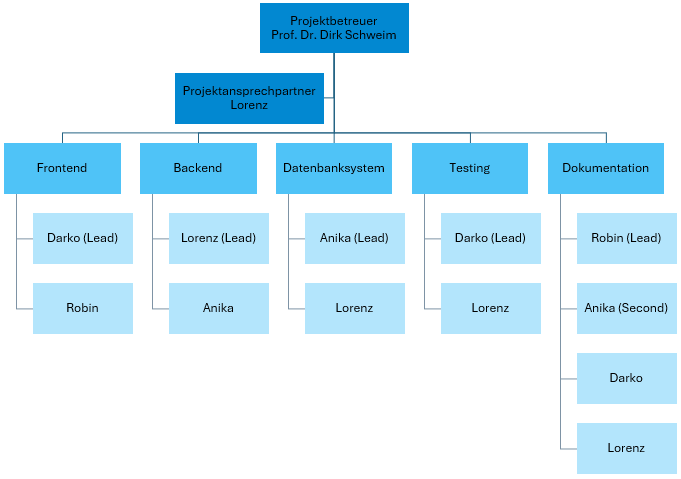
\includegraphics[width=0.8\textwidth]{organigramm}
    \caption{Organigramm}\label{fig:organigramm}
\end{figure}

Das Organigramm weist die Struktur und die Verantwortlichkeiten innerhalb des Projektteams auf.
Es gibt einen klaren Aufbau, der die verschiedenen Rollen und Zuständigkeiten verdeutlicht.

\begin{itemize}
    \item \textbf{Projektbetreuer:}
    \begin{itemize}
        \item \textbf{Prof. Dr. Dirk Schweim:} Der Projektbetreuer steht an oberster Stelle und ist für die Betreuung des Projekts verantwortlich.
    \end{itemize}

    \item \textbf{Projektansprechpartner:}
    \begin{itemize}
        \item \textbf{Lorenz:} Der Projektansprechpartner steht direkt unter dem Projektbetreuer und ist für die Koordination und Kommunikation innerhalb des Teams als auch zum Projektbetreuer zuständig.
    \end{itemize}

    \item \textbf{Frontend:}
    \begin{itemize}
        \item \textbf{Hauptverantwortlich:} Darko
        \item \textbf{Vertretend:} Robin
        \item Die Frontend-Sparte ist für die Gestaltung und Implementierung der Benutzeroberfläche zuständig.
        Darko ist hauptverantwortlich für diese Abteilung, unterstützt von Robin.
    \end{itemize}

    \item \textbf{Backend:}
    \begin{itemize}
        \item \textbf{Hauptverantwortlich:} Lorenz
        \item \textbf{Vertretend:} Anika
        \item Das Backend kümmert sich um die serverseitige Logik und Datenverarbeitung.
        Lorenz ist der Hauptverantwortliche, wobei Anika unterstützend tätig ist.
    \end{itemize}

    \item \textbf{Datenbanksystem:}
    \begin{itemize}
        \item \textbf{Hauptverantwortlich:} Anika
        \item \textbf{Vertretend:} Lorenz
        \item Diese Sparte ist für die Verwaltung und Wartung der Datenbank zuständig.
        Anika hat die Hauptverantwortung, unterstützt von Lorenz.
    \end{itemize}

    \item \textbf{Testing:}
    \begin{itemize}
        \item \textbf{Verantwortlich:} Darko, Lorenz
        \item Testing führt Tests durch, um die Qualität und Funktionalität der Plattform sicherzustellen.
        Darko und Lorenz teilen sich die Verantwortung in diesem Bereich.
    \end{itemize}

    \item \textbf{Dokumentation:}
    \begin{itemize}
        \item \textbf{Hauptverantwortlich:} Robin
        \item \textbf{Vertretend verantwortlich:} Anika
        \item \textbf{Weitere Beteiligte:} Darko, Lorenz
        \item Die Dokumentation wird von allen im Projektteam erstellt und gepflegt.
        Robin ist hauptverantwortlich, Anika übernimmt eine vertretende Rolle, während auch Darko und Lorenz aktiv mitwirken.
    \end{itemize}
\end{itemize}


Diese Struktur weist eine klare Rollenverteilung und entsprechende Vertretung auf, die dem Projektteam ermöglicht, effizient und effektiv an Aufgaben zu arbeiten und ermöglicht eine bessere Zusammenarbeit.



\subsection{Ablaufplanung (Gantt / Netzplan)}\label{subsec:ablaufplan}
Wird in YouTrack erstellt.

Lorenz ipsum dolor sit amet, consetetur sadipscing elitr, sed diam nonumy eirmod tempor invidunt ut labore et dolore magna aliquyam erat, sed diam voluptua.
At vero eos et accusam et justo duo dolores et ea rebum.
Stet clita kasd gubergren, no sea takimata sanctus est Lorem ipsum dolor sit amet.
Lorenz ipsum dolor sit amet, consetetur sadipscing elitr, sed diam nonumy eirmod tempor invidunt ut labore et dolore magna aliquyam erat, sed diam voluptua.
At vero eos et accusam et justo duo dolores et ea rebum.
Stet clita kasd gubergren, no sea takimata sanctus est Lorem ipsum dolor sit amet.
Lorenz ipsum dolor sit amet, consetetur sadipscing elitr, sed diam nonumy eirmod tempor invidunt ut labore et dolore magna aliquyam erat, sed diam voluptua.
At vero eos et accusam et justo duo dolores et ea rebum.
Stet clita kasd gubergren, no sea takimata sanctus est Lorem ipsum dolor sit amet.

\subsection{Stakeholder- und Risikoanalyse}\label{subsec:Stakeholder-Risikoanalyse}
Im Folgenden wurde eine Analyse bezüglich der Stakeholder des Projektes erstellt.
Diese haben unterschiedliche Vorstellungen, Einstellungen und Ansichten zum Projekt.
Ergänzend wurde auch eine Risikoanalyse erstellt, welche zur Übersicht von eventuell eintretenden Problemen verhilft. \par
\newpage %WICHTIG: Nur nötig wenn die Grafik bei der fertigen Doku NICHT unter den oberen Absatz passt! LaTeX schiebt sonst die Grafik weit unpassend im Text runter. @lorack do u know a fix? -Anika

%\Subsubsection{Stakeholderanalyse} \label{Stakeholderanalyse}

\begin{table}[h!]
    \centering
    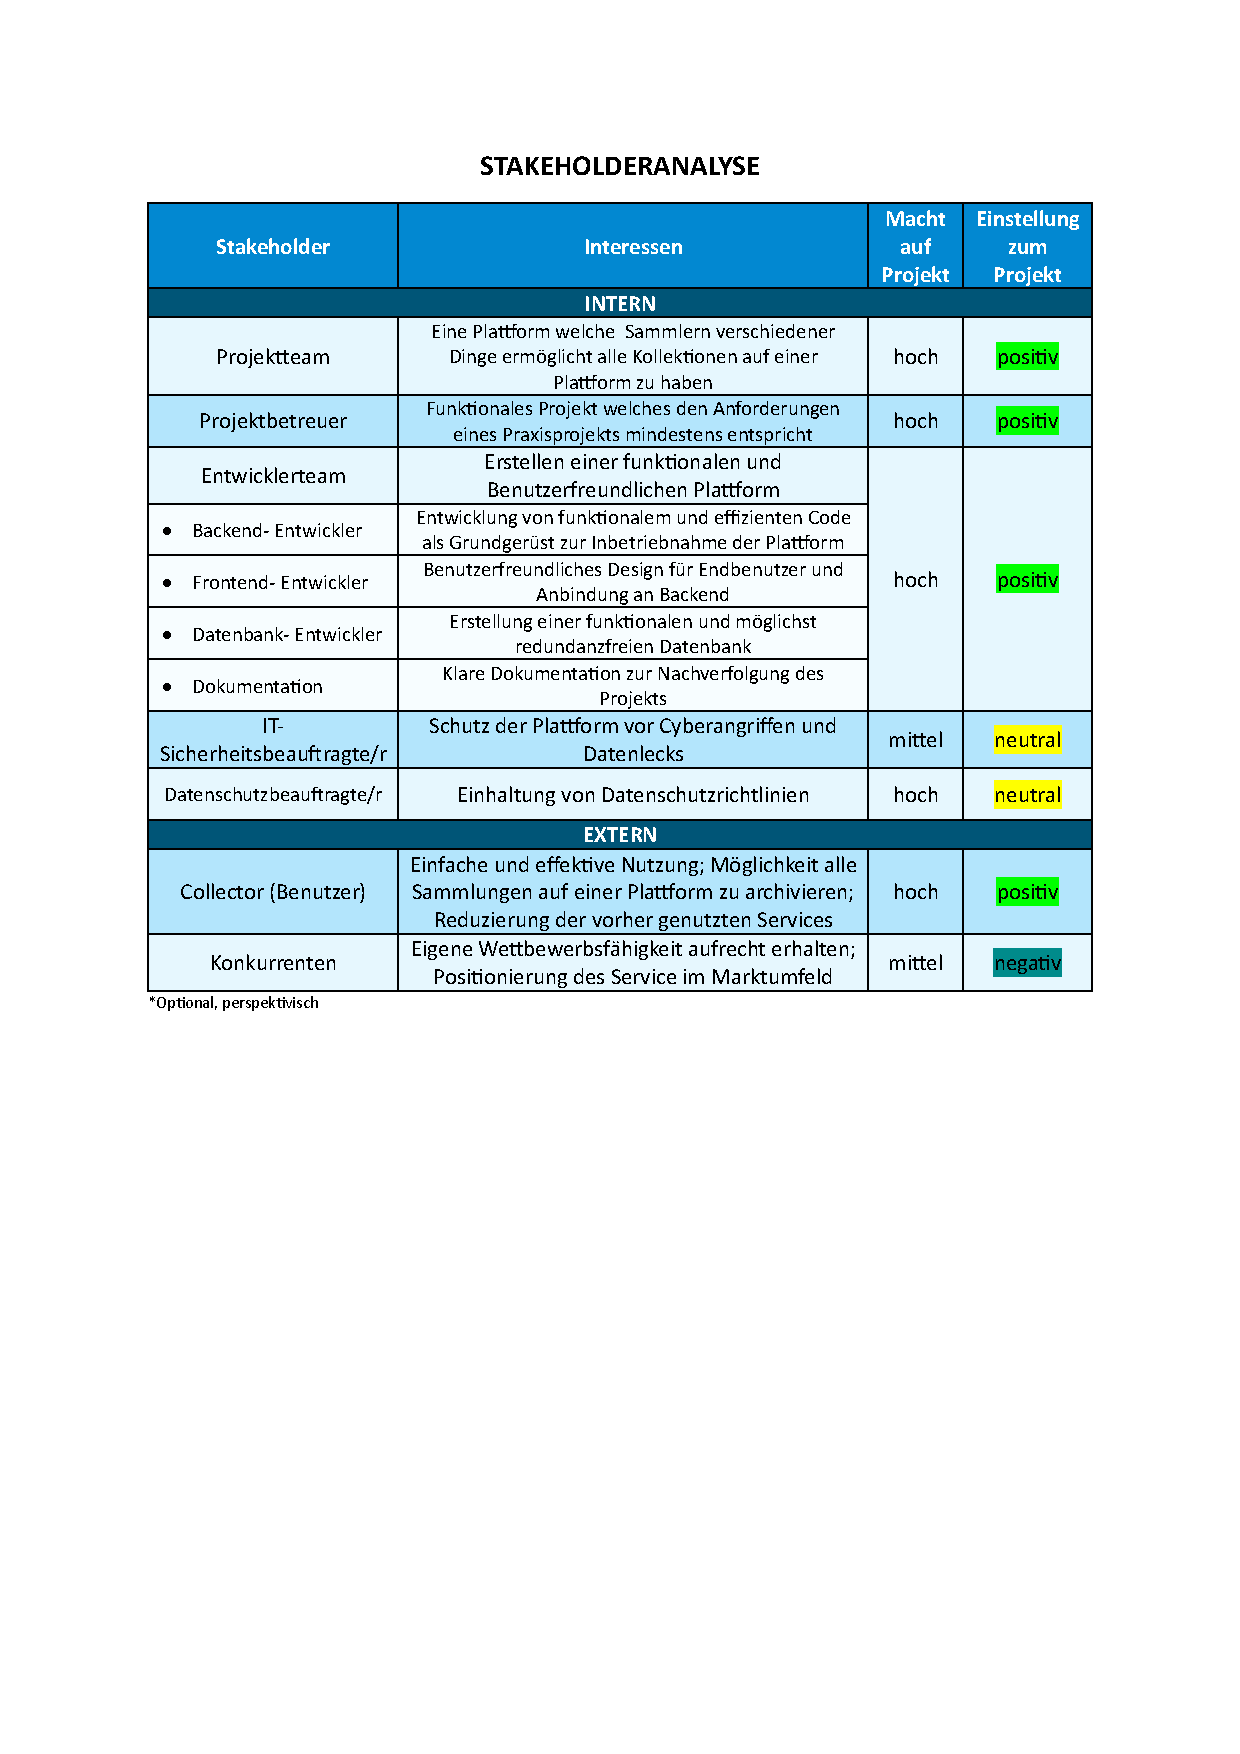
\includegraphics[width=\textwidth, clip, trim=1cm 14.5cm 1cm 3cm]{PM_SH_RISK_ANALYSIS}
    \caption{Stakeholderanalyse}\label{tab:stakegolderanalyse}
\end{table}

Das Projektteam besteht aus Studierenden, die im Rahmen ihres Studiums die Plattform entwickeln.
Das Hauptziel des Teams ist analog zur Zieldefinition von ~\ref{subsec:Zieldefinition}.
Rückblickend auf die Motivation in ~\ref{subsec:Motivation} ist das Team positiv eingestellt. \par

Der Projektbetreuer hat ein starkes Interesse daran, dass das Projekt den Anforderungen eines praxisnahen Studienprojekts entspricht.
Sein Fokus liegt darauf, dass das Projekt nicht nur funktional, sondern auch innovativ und praxisnah ist.
Er hat erheblichen Einfluss auf den Projektverlauf und unterstützt das Team mit wertvollem Feedback und fachlicher Anleitung. \par

Das Entwicklerteam, welches aus dem Projektteam besteht, ist in mehrere spezialisierte Gruppen unterteilt, analog zum Organigramm in ~\ref{subsec:Organigramm}.
Alle Entwicklergruppen haben parallel zum Projektteam-Stakeholder ein hohes Interesse am Projekterfolg und eine positive Einstellung zur Aufgabe, die einzelnen Interessen wurden zwecks persönlicher Lernerfolge nochmal aufgelistet. \par

Als weiterer Stakeholder erweist sich die Rolle der Datenschutzbeauftragten, dessen Hauptaufgabe darin besteht, die Einhaltung der Datenschutzrichtlinien sicherzustellen.
Diese Rolle hat einen hohen Einfluss auf das Projekt, da Datenschutz ein wesentliches, aber auch rechtliches Kriterium für die Plattform darstellt.
Entsprechend ist die Einstellung neutral gehalten. \par


Die Hauptnutzer der Plattform, die Sammler (Collector), stellen einen wesentlichen externen Stakeholder dar.
Ihr Interesse liegt in der einfachen und effektiven Nutzung der Plattform, die es ihnen ermöglicht, ihre Sammlungen zentral zu archivieren und die Nutzung mehrerer vorheriger Dienste zu reduzieren.
Ihre hohe Erwartung und positive Einstellung gegenüber der Plattform sind entscheidend für dessen Akzeptanz und Projekterfolg. \par

%\Subsubsection{Risikoanalyse} \label{Risikoanalyse}
%wichtig: Stake war in Präsens/Futur geschrieben, Risiko bewusst in Vergangenheitsform! >Discuss -Anika

\begin{table}[h!]
    \centering
    \includegraphics[page=2, width=\textwidth, clip, trim=1cm 20cm 1cm 4cm]{PM_SH_RISK_ANALYSIS}
    \caption{Risikoanalyse}\label{tab:risikoanalyse}
\end{table}

Die Entwicklung einer universellen Sammlerplattform wie Collectiqo wies verschiedene Risiken auf, die frühzeitig erkannt und gemindert wurden.
Eine gründliche Risikoanalyse ermöglichte es, potenzielle Herausforderungen zu identifizieren und geeignete Maßnahmen zu entwickeln, um den Projekterfolg sicherzustellen.

\begin{itemize}
    \item \textbf{Technische Herausforderungen:}

    Ein bedeutendes Risiko bei der Entwicklung von Collectiqo lag in der technischen Komplexität des Projekts.
    Da das Projektteam bisher andere Anwendungsfelder bedient hatte, musste das vorhandene Wissen für das Projekt angeglichen und ergänzt werden.
    Um dieses Risiko zu minimieren, war es wichtig, eine gründliche technische Analyse vor Beginn des Projekts durchzuführen.
    Das Projektteam definierte klare und detaillierte Anforderungen und zog so verschiedene technische Lösungen in Betracht, um die Lernkurve entsprechend auf einem möglichen Level, aber dennoch herausfordernd für den eigenen Lernerfolg zu halten.

    \item \textbf{Kommunikationsprobleme:}
    Ein weiteres erhebliches Risiko bestand in möglichen Kommunikationsproblemen innerhalb des Projektteams.
    Da die Teammitglieder verschiedene Arbeitsweisen und Entwicklerstandards ihrer Unternehmen und eigener Erfahrung gewohnt sind, hätte es zu Verständnisproblemen kommen können, welche potentiell zu Verzögerungen, Qualitätsproblemen und einem schlechten Arbeitsklima geführt hätten.
    Um dieses Risiko zu bewältigen, war eine klare und regelmäßige Kommunikation entscheidend.
    Entgegenwirkend hielt das Team regelmäßige Meetings und verwendete YouTrack, um den Fortschritt zu verfolgen und sicherzustellen, dass alle Mitglieder auf dem gleichen Stand sind.

    \item \textbf{Verfügbarkeitsprobleme:}
    Ein weiteres Risiko bestand in möglichen Verfügbarkeitsproblemen, wie dem Ausfall von Services oder Hardware.
    Die Eintrittswahrscheinlichkeit wurde als mittel eingestuft, aber die Auswirkungen könnten den Projektfortschritt erheblich behindern.
    Um dieses Risiko zu minimieren, wurden Fall-Back-Alternativen und Lokalkopien erstellt, um die Arbeit auch bei Ausfällen fortsetzen zu können.
\end{itemize}



\subsection{Kosten- und Aufwandsplanung}\label{subsec:Kosten-Aufwandsplanung}
Lorenz ipsum dolor sit amet, consetetur sadipscing elitr, sed diam nonumy eirmod tempor invidunt ut labore et dolore magna aliquyam erat, sed diam voluptua.
At vero eos et accusam et justo duo dolores et ea rebum.
Stet clita kasd gubergren, no sea takimata sanctus est Lorem ipsum dolor sit amet.
Lorenz ipsum dolor sit amet, consetetur sadipscing elitr, sed diam nonumy eirmod tempor invidunt ut labore et dolore magna aliquyam erat, sed diam voluptua.
At vero eos et accusam et justo duo dolores et ea rebum.
Stet clita kasd gubergren, no sea takimata sanctus est Lorem ipsum dolor sit amet.
Lorenz ipsum dolor sit amet, consetetur sadipscing elitr, sed diam nonumy eirmod tempor invidunt ut labore et dolore magna aliquyam erat, sed diam voluptua.
At vero eos et accusam et justo duo dolores et ea rebum.
Stet clita kasd gubergren, no sea takimata sanctus est Lorem ipsum dolor sit amet.

\subsection{Tools}\label{subsec:Tools}
Lorenz ipsum dolor sit amet, consetetur sadipscing elitr, sed diam nonumy eirmod tempor invidunt ut labore et dolore magna aliquyam erat, sed diam voluptua.
At vero eos et accusam et justo duo dolores et ea rebum.
Stet clita kasd gubergren, no sea takimata sanctus est Lorem ipsum dolor sit amet.
Lorenz ipsum dolor sit amet, consetetur sadipscing elitr, sed diam nonumy eirmod tempor invidunt ut labore et dolore magna aliquyam erat, sed diam voluptua.
At vero eos et accusam et justo duo dolores et ea rebum.
Stet clita kasd gubergren, no sea takimata sanctus est Lorem ipsum dolor sit amet.
Lorenz ipsum dolor sit amet, consetetur sadipscing elitr, sed diam nonumy eirmod tempor invidunt ut labore et dolore magna aliquyam erat, sed diam voluptua.
At vero eos et accusam et justo duo dolores et ea rebum.
Stet clita kasd gubergren, no sea takimata sanctus est Lorem ipsum dolor sit amet.

\begin{itemize}
    \item one
    \item two
    \item three
\end{itemize}
